\documentclass[../main.tex]{subfiles}
\begin{document}
\chapter{Lecture 7 - 30-03-2020}
Bounding statistical risk of a predictor\\\
Design a learning algorithm that predict with small statistical risk\\
$$
(D,\ell) \qquad \ell_d(h) = \barra{E}\left[ \, \ell (y), h(x) \, \right]
$$
were $D$ is unknown
$$
\ell(y, \hat{y}) \in [0,1] \quad \forall y, \hat{y} \in Y
$$
We cannot compute statistical risk of all predictor.\\
We assume statistical loss is bounded so between 0 and 1. Not true for all
losses (like logarithmic ).\\
Before design a learning algorithm with lowest risk, How can we estimate
risk?\\
We can use test error $\rightarrow$ way to measure performances of a predictor h.
We want to link test error and risk.
\\
Test set $S' = \{ (x'_1, y'_1) ...(x'_n,y'_n) \}$ is a random sample from $D$
\\
How can we use this assumption?\\
Go back to the definition of test error\\
\\
\red{ Sample mean (IT: Media campionaria)}\\
$$
\hat{\ell}_s(h) = \frac{1}{n} \cdot \sum_{t=1}^{n} \ell (\hat{y}_t,h(x'_t))
$$
i can look at this as a random variable
\col{$\ell(y'_t,h(x'_t))$}{Blue}
\\
$$
\barra{E} \left[ \, \ell (y'_t, h(x'_t)) \right] = \ell_D(h) \longrightarrow \red{risk}
$$\\
Using law of large number (LLN), i know that:
$$
\hat{\ell} \longrightarrow \ell_D(h) \qquad as \quad n \rightarrow \infty
$$
We cannot have a sample of $n = \infty$ so we will introduce another assumption:
the \red{Chernoff-Hoffding bound}

\section{Chernoff-Hoffding bound}
$$
Z_1,...,Z_n \quad \textit{iid random variable} \qquad \barra{E}\left[Z_t \right] = u
$$
all drawn for the same distribution 
\\
$$
t = 1, ..., n \qquad and \qquad 0 \leq Z_t \leq 1 \qquad t = 1,...,n \quad then \quad \forall \varepsilon > 0
$$\
$$
\barra{P} \left( \frac{1}{n} \cdot \sum_{t=1}^{n} z_t > u + \varepsilon \right) \leq e^{-2 \, \varepsilon^2 \, n} \qquad  or \qquad \barra{P} \left( \frac{1}{n} \cdot \sum_{t=1}^{n} z_t < u + \varepsilon \right) \leq e^{-2 \, \varepsilon^2 \, n}
$$
as sample size then $\downarrow$
$$
Z_t = \ell(Y'_t, h(X'_t)) \in \left[0,1\right]
$$
$
(X'_1, Y'_1)...(X'_n, Y'_N)$ are $iid$ therefore, \\ $\ell\left(Y'_t, h\left(X'_t\right)\right)$ \quad $t = 1,...,n $ \quad are also $iid$
\\
We are using the bound of e to bound the deviation of this.

\section{Union Bound}
Union bound: a collection of event not necessary disjoint, then i know
that probability of the union of this event is the at most the sum of the
probabilities of individual events
$$
A_1, ..., A_n \qquad \barra{P}\left( A_1 \cup ... \cup A_n \right) \leq \sum_{t=1}^{n} \barra{P} \left(A_t\right)
$$
\begin{figure}[h]
    \centering
    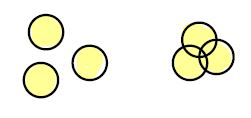
\includegraphics[width=0.3\linewidth]{../img/lez7-img1.JPG}
    \caption{Example}
    %\label{fig:}
\end{figure}\\
\red{that's why $ \leq$}
\\\\
$$
\barra{P} \left(|\,\hat{\ell}_{s'} \left( h \right) - \ell_D\left( h \right) \, | \, > \varepsilon \right)
$$
This is the probability according to the random draw of the test set.\\
\\
If test error differ from the risk by a number epsilon > 0. I want to bound the
probability. This two thing will differ by more than epsilon. How can i use the
Chernoff bound?
$$
|\,\hat{\ell}_{s'} \left( h \right) - \ell_D\left( h \right) \, | \, > \varepsilon  \quad \Rightarrow \quad 
\hat{\ell}_{s'}\left(h\right)-\ell_D\left(h\right) > \varepsilon \quad \vee \quad
\hat{\ell}_D \left(h\right)-\ell_{s'}\left(h\right) > \varepsilon
$$

$$
A, B \qquad A \Rightarrow B \qquad \barra{P} \left( A \right) < \barra{P} \left( B \right)
$$
\begin{figure}[h]
    \centering
    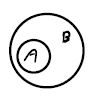
\includegraphics[width=0.2\linewidth]{../img/lez7-img2.JPG}
    \caption{Example}
    %\label{fig:}
\end{figure}
$$
\barra{P} \left(|\,\hat{\ell}_{s'} \left( h \right) - \ell_D\left( h \right) \, | \, > \varepsilon \right) 
\leq
\barra{P} \left( \,| \hat{\ell}_{s'}\left(h\right)-\ell_D\left(h\right) |\,\right) \quad
\cup \quad
\barra{P} \left( \,|
\hat{\ell}_D \left(h\right)-\ell_{s'}\left(h\right) 
|\,\right) 
\leq
$$\
$$
\leq
\barra{P} \left( \hat{\ell}_{s'} > \ell_D\left(h\right) + \varepsilon \right) + \barra{P} \left( \hat{\ell}_{s'} < \ell_D\left(h\right) - \varepsilon \right) 
\quad
\leq \quad
2 \cdot e^{-2 \, \varepsilon^2 \, n} \quad \Rightarrow \red{ \textit{we call it } \delta }
$$
$$
\varepsilon = \sqrt[]{\frac{1}{2\cdot n}\ln \frac{2}{\delta
}}
$$
\col{The two events are disjoint}{Blue}\\\\
This mean that probability of this deviation is at least delta!
$$
|\, \hat{\ell}_{s'}\left(h\right)-\ell_D\left(h\right) \, | \leq \sqrt[]{\frac{1}{2\cdot n} \ln \frac{2}{\delta}} \qquad \textit{with probability at least $1- \delta$}
$$
\red{Test error of true estimate is going to be good for this value ($\delta$)}
\\
\begin{figure}[h]
    \centering
    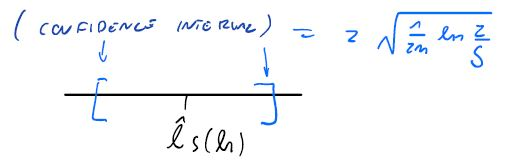
\includegraphics[width=0.5\linewidth]{../img/lez7-img3.JPG}
    \caption{Example}
    %\label{fig:}
\end{figure}Confidence interval for risk at confidence level 1-delta.\\
I want to take $\delta = 0,05$ so that $1 - \delta$ is $95\%$. So test error is going to be
an estimate of the true risk which is precise that depend on how big is the test
set ($n$).\\
As n grows I can pin down the position of the true risk.\\\
This is how we can use probability to make sense of what we do in practise.
If we take a predictor h we can compute the risk error estimate.\\
We can measure how accurate is our risk error estimate.\\
\textbf{Test error is an estimate of risk for a given predictor (h).}
\\ 
$$
\barra{E} \left[ \, \ell\left( Y'_t, h\left(X'_t\right)\right) \, \right] = \ell_D \left( h\right) 
$$
\textbf{h is fixed with respect to S’} $\longrightarrow$ $h$ does not depend on the test set.
So learning algorithm which produce h not have access to test set.\\
If we use test set we break down this equation.
\\\\
Now, how to \textbf{build a good algorithm?}\\
Training set $S = \{ \left(x_1,y_1\right)...\left(x_m,y_m\right) \}$ random sample
\\$ A $ \qquad $A\left(S\right) = h $ predictor output by $A$ given $S$
where A is \red{learning algorithm as function of traning set $S$.}
\\
$\forall \, S$ \qquad $A\left(S\right) \in H \qquad h^* \in H $
\\
$$
\ell_D\left(h^*\right) = min \, \ell_D \left(h\right) \qquad \hat{\ell}_s\left(h^*\right) \textit{is closed to } \ell_D\left(h^*\right) \longrightarrow \textbf{it is going to have small error }
$$
where $\ell_D\left(h^*\right)$ is the \red{training error of $h^*$}
\begin{figure}[h]
    \centering
    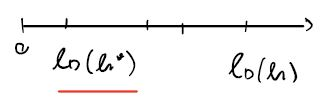
\includegraphics[width=0.3\linewidth]{../img/lez7-img4.JPG}
    \caption{Example}
    %\label{fig:}
\end{figure}\\
This guy $\ell_D\left(h^*\right)$ is closest to $0$ since optimum\\
\begin{figure}[h]
    \centering
    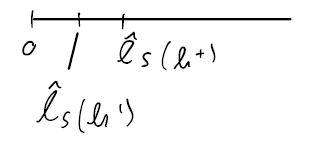
\includegraphics[width=0.3\linewidth]{../img/lez7-img5.JPG}
    \caption{Example}
    %\label{fig:}
\end{figure}\\
In risk we get opt in $h^*$ but in empirical one we could get another $h’$ better than $h^+$
\\\\
In order to fix on a concrete algorithm we are going to take the empirical Islam
minimiser (ERM) algorithm.
\\
$A$ is $ERM$ on $H$ \qquad $\left(A\right) = \hat{h} = (\in) \, argmin \, \hat{\ell}_S\left(h\right)
$
\\
Once I piack $\hat{h}$ i can look at training error of ERM
\\
$$ \hat{\ell}_S\left(\hat{h}\right) of \hat{h} = A(S)$$
where $\hat{\ell}_S$ is the training error
\\\\
Should $\hat{\ell}_S\left(\hat{h}\right)$ be close to $\ell_D\left(\hat{h}\right)$ ?
\\
I’m interested in empirical error minimiser and do a trivial decomposition.
\\\\
$$
\ell_d\left(\hat{h}\right) = \quad \ell_D\left(\hat{h}\right) - \ell_d\left(h^*\right) + \qquad \longrightarrow \red{\textbf{ Variance error $\Rightarrow$ Overfitting}}
$$
$$
\qquad \quad +\,  \ell_d\left(h^+\right) - \ell_d\left(f^*\right) + \qquad \longrightarrow \red{\textbf{ Bias error $\Rightarrow$ Underfitting}}
$$
$$ \qquad \qquad \quad 
+ \, \ell_D\left(f^*\right)\qquad \qquad \quad  \longrightarrow \red{\textbf{ Bayes risk $\Rightarrow$ Unavoidable}} 
$$\\
Even the best predictor is going to suffer that\\
$$ f^* \textit{ is \textbf{Bayes Optimal} for $(D,\ell)$ }
$$
$$\forall \, h \qquad \ell_D\left(h\right) \geq \ell_D\left(f^*\right)
$$
If $f^* \not\in H$ then $\ell_D\left(h^*\right) > \ell_D (f^*) $
\\\\
If i pick $h^*$ I will pick some error because we are not close enough to the risk.\\
We called this component \red{\textbf{bias error}}.\\
Bias error is responsible for underfitting (when training and test are close
to each but they are both high :( )\\
\red{\textbf{Variance error}} over fitting
\\
\begin{figure}[h]
    \centering
    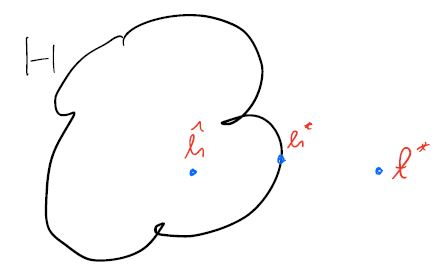
\includegraphics[width=0.5\linewidth]{../img/lez7-img6.JPG}
    \caption{Draw of how $\hat{h}$, $h^*$ and $f^*$ are represented}
    %\label{fig:}
\end{figure}\\
Variance is a random quantity and we want to study this.
We can always get risk from training error.
\\\\
\section{Studying overfitting of a ERM}
We can bound it with probability.\\
\bred{I add and subtract trivial traning error $\hat{\ell}_S\left(h\right)$}
$$
\ell_D \left(\hat{h}\right) 
-\ell_d \left(h^*\right)
\quad
 = 
 \quad 
\ell_D \left(\hat{h}\right) - 
\hat{\ell}_S\left( h \right)
+ 
\hat{\ell}_S \left( \hat{h} \right)
- \ell_D\left( h^* \right) \leq 
$$
$$
\leq \, \ell_D \left(\hat{h}\right) - 
\hat{\ell}_S\left( \hat{h} \right)
+ 
\hat{\ell}_S \left( h^* \right)
- \ell_D\left( h^* \right) \leq \,
$$
$$
\leq \, | \, \ell_D\left(\hat{h}\right) - \hat{\ell}_S\left(h\right) \, | + | \, \hat{\ell}_S\left(h^+\right) - \ell_D\left(h^*\right) \, |\, \leq
$$
$$
\leq \quad 2 \cdot max \, |\hat{\ell}_S\left(h\right) - \ell_D\left(h\right) |
$$
(no probability here)\\
\textbf{Any given $\hat{h}$ minising $\hat{\ell}_S\left(h\right)$}
\\\\
Now assume we have a large deviation
\\
$$
\textit{Assume \quad } \ell_D\left(\hat{h}\right) - \ell_D \left(h^* \right) > \varepsilon \qquad \Rightarrow \qquad max \, | \, \hat{\ell}_S\left(h\right) - \ell_D \left(h\right) \, | > \frac{\varepsilon}{2}
$$
\\
We know $\ell_d\left(\hat{h}\right) - \ell_D\left(h^*\right) 
\quad \leq \quad 2
 \cdot max \,|\, \hat{\ell}_S \left(h\right) - \ell_D\left(h\right) \, |$ \quad $\Rightarrow$
\\
$$
\Rightarrow \quad \exists h \in H \qquad | \, \hat{\ell}_S\left(h\right) - \ell_D\left(h \right) \, | \, > \frac{3}{2} \qquad \Rightarrow
$$
with $|H| < \infty$
$$
\Rightarrow U \left( \, | \, \hat{\ell}_S\left(h\right) - \ell_D \left(h\right) \, | \, \right) > \frac{3}{2}
$$
\\
$$
\barra{P} \left( \ell_D \left(\hat{h}\right) - \ell_D \left( h^* \right) 
> 
\varepsilon \right) \quad \leq \quad \barra{P} \left( U \left( \, | \, \hat{\ell}_S\left(h\right) - \ell_D \left(h\right) \, | \, \right) > \frac{3}{2} \right) \quad \leq
$$
$$
\red{\leq}  \quad \sum_{h \in H}{} \, \barra{P} \left( \,  | \, \hat{\ell}_S\left(h\right) - \ell_D \left(h\right) \, |  \, > \frac{3}{2}  \right) \qquad \leq \qquad \sum_{h \in H}{} 2 \cdot e^{-2 \, \left(\frac{\varepsilon}{2}\right)^2 \, m} \qquad \leq 
$$
\bred{Union Bound } \blue{Chernoff. Hoffding bound ($\barra{P} \left( ... \right) $)}
$$
\leq \quad 2 \cdot |H| e^{- \, \frac{\varepsilon^2}{2} \, m}
$$
\\ 
Solve for $\varepsilon$ \qquad
$
2 \cdot |H| e^{- \, \frac{\varepsilon^2}{2} \, m} \quad = \quad \delta
$
$$
\textit{ Solve for } \varepsilon \longrightarrow \quad  \varepsilon = \sqrt[]{\frac{2}{m} \cdot \ln \cdot \frac{2|H|}{\delta}}
$$
$$
\ell_D\left(\hat{h}\right) - \ell_D \left( h^* \right) \quad\leq \quad \sqrt[]{\frac{2}{m} \cdot \ln \cdot \frac{2|H|}{\delta}}
$$
\\
With probability at least $1 - \delta$ with respect to random draw of $S$.\\
We want $m >> ln |H|$ \quad $\longrightarrow$ in order to avoid overfitting
\\
\end{document}